\documentclass[aspectratio=169,10pt]{beamer}

\usepackage[T1]{fontenc}
\usepackage[utf8]{inputenc}
\usepackage{lmodern}
\usepackage{graphicx}
\usepackage{booktabs}
\usepackage{amsmath}
\usepackage{tikz}
\usetikzlibrary{arrows.meta,positioning}

\graphicspath{{../figures/}{figures/}}

\definecolor{Ink}{HTML}{102A43}
\definecolor{DeepTeal}{HTML}{0B5563}
\definecolor{SoftTeal}{HTML}{D8EEF0}
\definecolor{WarmAmber}{HTML}{C88719}
\definecolor{Paper}{HTML}{FAF7EF}
\definecolor{Muted}{HTML}{52616B}

\setbeamercolor{normal text}{fg=Ink,bg=Paper}
\setbeamercolor{frametitle}{fg=Ink,bg=Paper}
\setbeamercolor{title}{fg=Ink}
\setbeamercolor{subtitle}{fg=DeepTeal}
\setbeamercolor{structure}{fg=DeepTeal}
\setbeamercolor{block title}{fg=Paper,bg=DeepTeal}
\setbeamercolor{block body}{fg=Ink,bg=SoftTeal}

\setbeamertemplate{navigation symbols}{}
\setbeamertemplate{frametitle}{
  \vspace{0.35cm}
  \begin{beamercolorbox}[wd=\paperwidth,leftskip=0.65cm,rightskip=0.65cm]{frametitle}
    \usebeamerfont{frametitle}\insertframetitle
  \end{beamercolorbox}
  \vspace{-0.25cm}
  \hspace{0.65cm}{\color{WarmAmber}\rule{0.86\paperwidth}{0.7pt}}
}
\setbeamertemplate{footline}{
  \hfill
  \color{Muted}\scriptsize
  \ifnum\value{framenumber}<8
    \insertframenumber/7
  \else
    Anexo
  \fi
  \hspace{0.45cm}\vspace{0.22cm}
}

\newcommand{\highlight}[1]{\textcolor{DeepTeal}{\textbf{#1}}}
\newcommand{\smallnote}[1]{{\scriptsize\textcolor{Muted}{#1}}}

\title{Segmentaci\'on de Clientes Mayoristas}
\subtitle{Aprendizaje no supervisado para decisiones comerciales}
\author{Federico Mor\'an y Juan Barboza}
\date{Trabajo Pr\'actico Final - Aprendizaje No Supervisado}

\begin{document}

% Guion: abrir con el problema de negocio, no con el algoritmo.
\begin{frame}[plain]
  \vspace{0.25cm}
  {\Large\bfseries\color{Ink}\inserttitle}\\[0.1cm]
  {\color{DeepTeal}\insertsubtitle}\\[0.35cm]
  {\small \insertauthor}\\[0.1cm]
  {\scriptsize\color{Muted}\insertdate}

  \vfill
  \begin{columns}[T,onlytextwidth]
    \begin{column}{0.52\textwidth}
      \begin{block}{Pregunta}
        \large
        \textbf{?`Qu\'e grupos de clientes emergen a partir de su patr\'on de gasto anual?}
      \end{block}
    \end{column}
    \begin{column}{0.43\textwidth}
      \begin{itemize}
        \item No hay etiqueta de segmento.
        \item La cartera mezcla Horeca y Retail.
        \item Buscamos segmentos \highlight{interpretables y accionables}.
      \end{itemize}
    \end{column}
  \end{columns}

  \vfill
  \smallnote{Idea central: convertir patrones de compra en grupos \'utiles para log\'istica, precios, retenci\'on y venta cruzada.}
\end{frame}

% Guion: dejar explicito que las categoricas se reservan para validar, no para entrenar.
\begin{frame}{Dataset: atributos y validaci\'on externa}
  \begin{columns}[T,onlytextwidth]
    \begin{column}{0.42\textwidth}
      \begin{itemize}
        \item \highlight{Wholesale Customers} - UCI. 440 clientes mayoristas.
        \item Se agrupa \emph{solo} con las 6 variables de gasto anual: Fresh, Milk, Grocery, Frozen, Detergents\_Paper, Delicassen.
      \end{itemize}
      \vspace{0.1cm}
      \begin{block}{Validaci\'on externa (no son atributos)}
        \footnotesize
        \highlight{Channel} (Horeca / Retail): pseudo-etiqueta para las m\'etricas ARI y NMI.\\[0.08cm]
        \highlight{Region} (Lisboa / Oporto / otra): se inspecciona en t-SNE para descartar estructura geogr\'afica.\\[0.08cm]
        \smallnote{Se reservan \emph{fuera} del entrenamiento: usarlas como atributo har\'ia circular la validaci\'on.}
      \end{block}
    \end{column}
    \begin{column}{0.55\textwidth}
      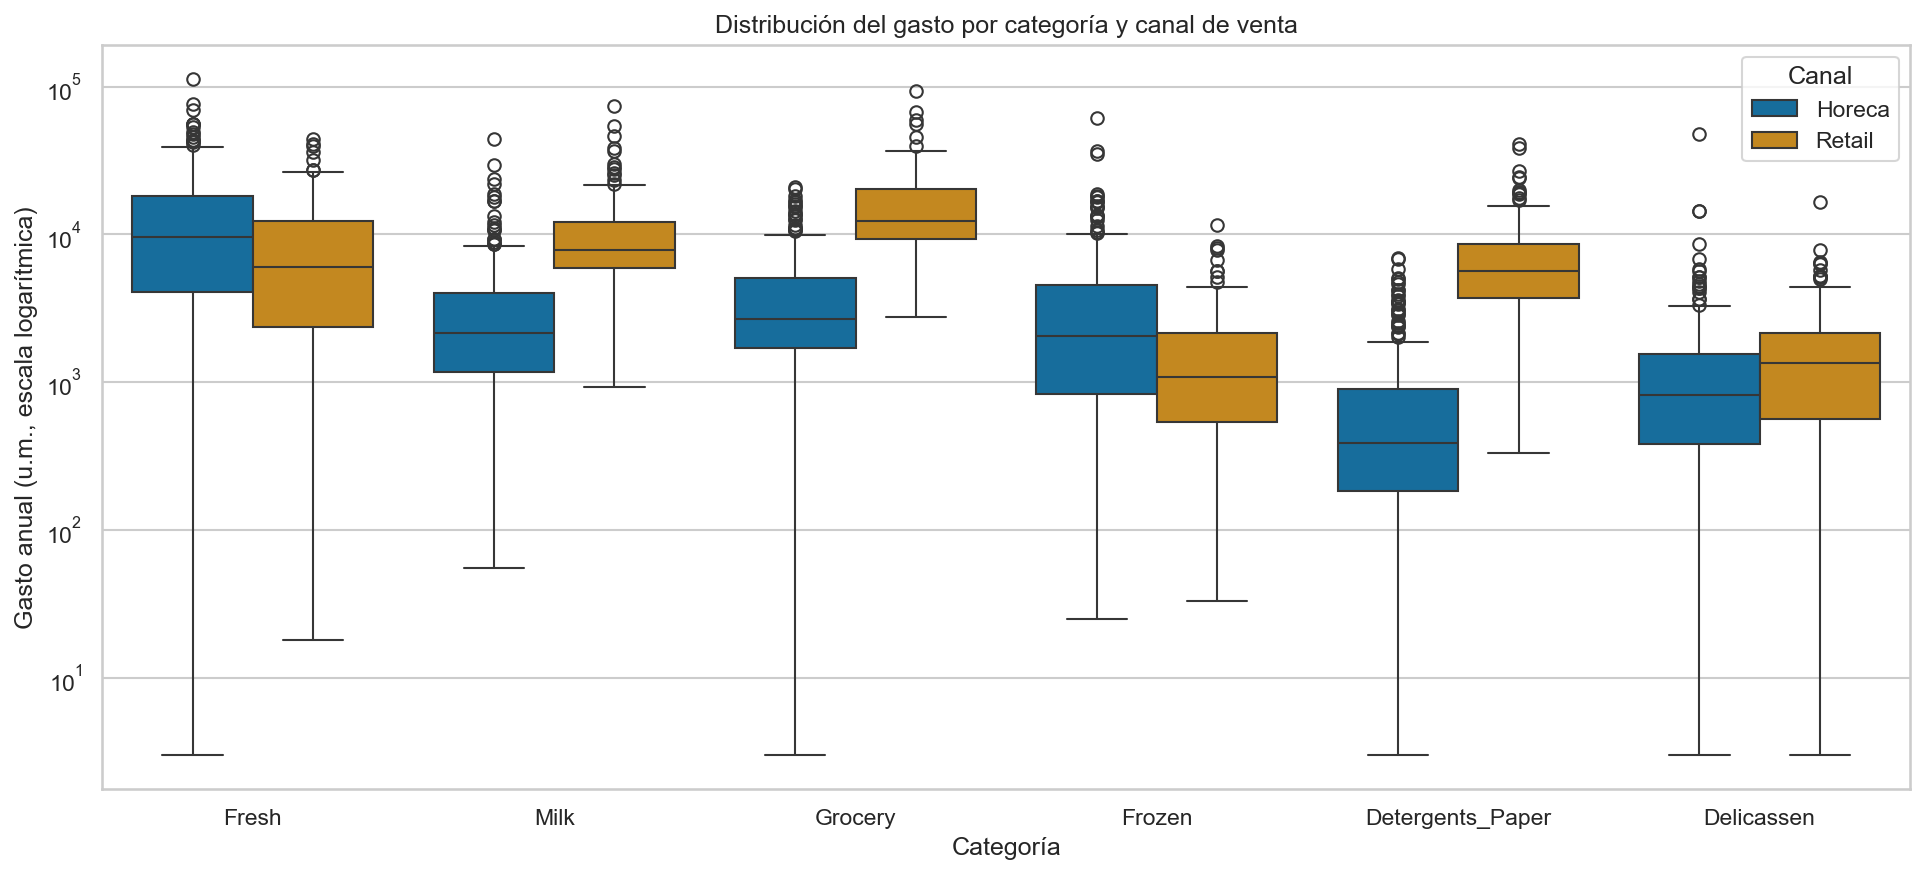
\includegraphics[width=\linewidth]{eda_gasto_por_canal.png}
      \vspace{0.05cm}
      \smallnote{Se\~nal EDA: Retail concentra m\'as Grocery, Milk y Detergents\_Paper; Horeca pesa m\'as en Fresh y Frozen. Anticipa que la estructura dominante se alinear\'a con el canal.}
    \end{column}
  \end{columns}
\end{frame}

% Guion: no explicar matematicamente cada algoritmo; contar decisiones y comparacion justa.
\begin{frame}{M\'etodo: pipeline simple y comparable}
  \centering
  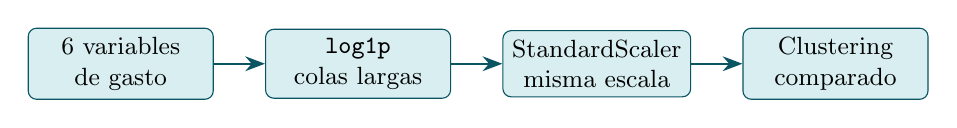
\begin{tikzpicture}[
    node distance=0.65cm,
    box/.style={draw=DeepTeal, fill=SoftTeal, rounded corners=3pt, minimum width=2.35cm, minimum height=0.8cm, align=center, font=\small},
    arrow/.style={-{Stealth[length=2.5mm]}, thick, color=DeepTeal}
  ]
    \node[box] (select) {6 variables\\de gasto};
    \node[box, right=of select] (log) {\texttt{log1p}\\colas largas};
    \node[box, right=of log] (scale) {StandardScaler\\misma escala};
    \node[box, right=of scale] (models) {Clustering\\comparado};
    \draw[arrow] (select) -- (log);
    \draw[arrow] (log) -- (scale);
    \draw[arrow] (scale) -- (models);
  \end{tikzpicture}

  \vspace{0.45cm}
  \begin{columns}[T,onlytextwidth]
    \begin{column}{0.49\textwidth}
      \begin{block}{Modelos}
        \begin{itemize}
          \item K-Means como referencia.
          \item Agglomerative Clustering.
          \item Gaussian Mixture Models.
          \item Deep Embedded Clustering.
        \end{itemize}
      \end{block}
    \end{column}
    \begin{column}{0.49\textwidth}
      \begin{block}{Evaluaci\'on}
        \begin{itemize}
          \item Interna: Silhouette, Davies-Bouldin, Calinski-Harabasz.
          \item Externa: Channel como pseudo-etiqueta (ARI, NMI).
          \item Outliers conservados: son clientes reales.
        \end{itemize}
      \end{block}
    \end{column}
  \end{columns}
\end{frame}

% Guion: un modelo por bloque; que aporta cada uno mas alla del baseline.
\begin{frame}{Tres modelos m\'as all\'a del baseline}
  \begin{columns}[T,onlytextwidth]
    \begin{column}{0.32\textwidth}
      \begin{block}{Agglomerative}
        \footnotesize
        \textbf{Jer\'arquico.} Cada cliente inicia como un grupo; se fusionan los m\'as cercanos. Enlace \highlight{Ward}: minimiza la varianza intra-grupo.\\[0.15cm]
        \smallnote{Elecci\'on: dendrograma + grilla de linkage $\Rightarrow$ k=3.}\\[0.12cm]
        \emph{Aporta:} jerarqu\'ia interpretable; no exige grupos esf\'ericos.
      \end{block}
    \end{column}
    \begin{column}{0.32\textwidth}
      \begin{block}{Gaussian Mixture}
        \footnotesize
        \textbf{Probabil\'istico.} Mezcla de $k$ gaussianas (EM); cada cliente recibe una \highlight{probabilidad} de pertenencia (asignaci\'on blanda).\\[0.15cm]
        \smallnote{Elecci\'on: BIC sobre covarianza $\times$ k $\Rightarrow$ full, k=3.}\\[0.12cm]
        \emph{Aporta:} cuantifica la incertidumbre $\to$ clientes fronterizos.
      \end{block}
    \end{column}
    \begin{column}{0.32\textwidth}
      \begin{block}{Deep Embedded Clustering}
        \footnotesize
        \textbf{Deep clustering.} Un autoencoder aprende una \highlight{representaci\'on latente} y una capa de agrupamiento se optimiza junto al encoder (KL).\\[0.15cm]
        \smallnote{Elecci\'on: grilla $d_{\mathrm{lat}}\times k$, m\'etricas internas.}\\[0.12cm]
        \emph{Aporta:} captura no-linealidad; pensado para alta dimensi\'on.
      \end{block}
    \end{column}
  \end{columns}
  \vspace{0.25cm}
  \smallnote{K-Means queda como \emph{baseline} de referencia.}
\end{frame}

% Guion: la tabla no es para leer todo; marcar que Ward gana por interpretabilidad.
\begin{frame}{Resultados: estructura recuperada sin etiquetas}
  \begin{columns}[T,onlytextwidth]
    \begin{column}{0.58\textwidth}
      \begin{table}
        \centering
        \scriptsize
        \begin{tabular}{lccc}
          \toprule
          M\'etodo & Silhouette & ARI canal & NMI canal \\
          \midrule
          K-Means (k=2) & \textbf{0.290} & 0.514 & 0.445 \\
          Ward (k=3) & 0.255 & \textbf{0.549} & 0.409 \\
          GMM (k=3) & 0.239 & 0.431 & 0.379 \\
          DEC (k=2) & 0.285 & 0.546 & \textbf{0.457} \\
          \bottomrule
        \end{tabular}
      \end{table}
    \end{column}
    \begin{column}{0.38\textwidth}
      \begin{block}{Lectura}
        \begin{itemize}
          \item Todos los m\'etodos encuentran estructura real.
          \item La estructura se alinea con canal, pero no se reduce solo a canal.
          \item \highlight{Ward k=3} ofrece la partici\'on m\'as \'util para negocio.
        \end{itemize}
      \end{block}
    \end{column}
  \end{columns}

  \vspace{0.25cm}
  \smallnote{La decisi\'on no se toma por una \'unica m\'etrica: se combina calidad num\'erica, tama\~nos de grupos e interpretabilidad.}
\end{frame}

% Guion: puente visual entre metricas e insight; el t-SNE explica por que las silhouettes son moderadas.
\begin{frame}{Visualizaci\'on t-SNE: qu\'e ven los modelos}
  \centering
  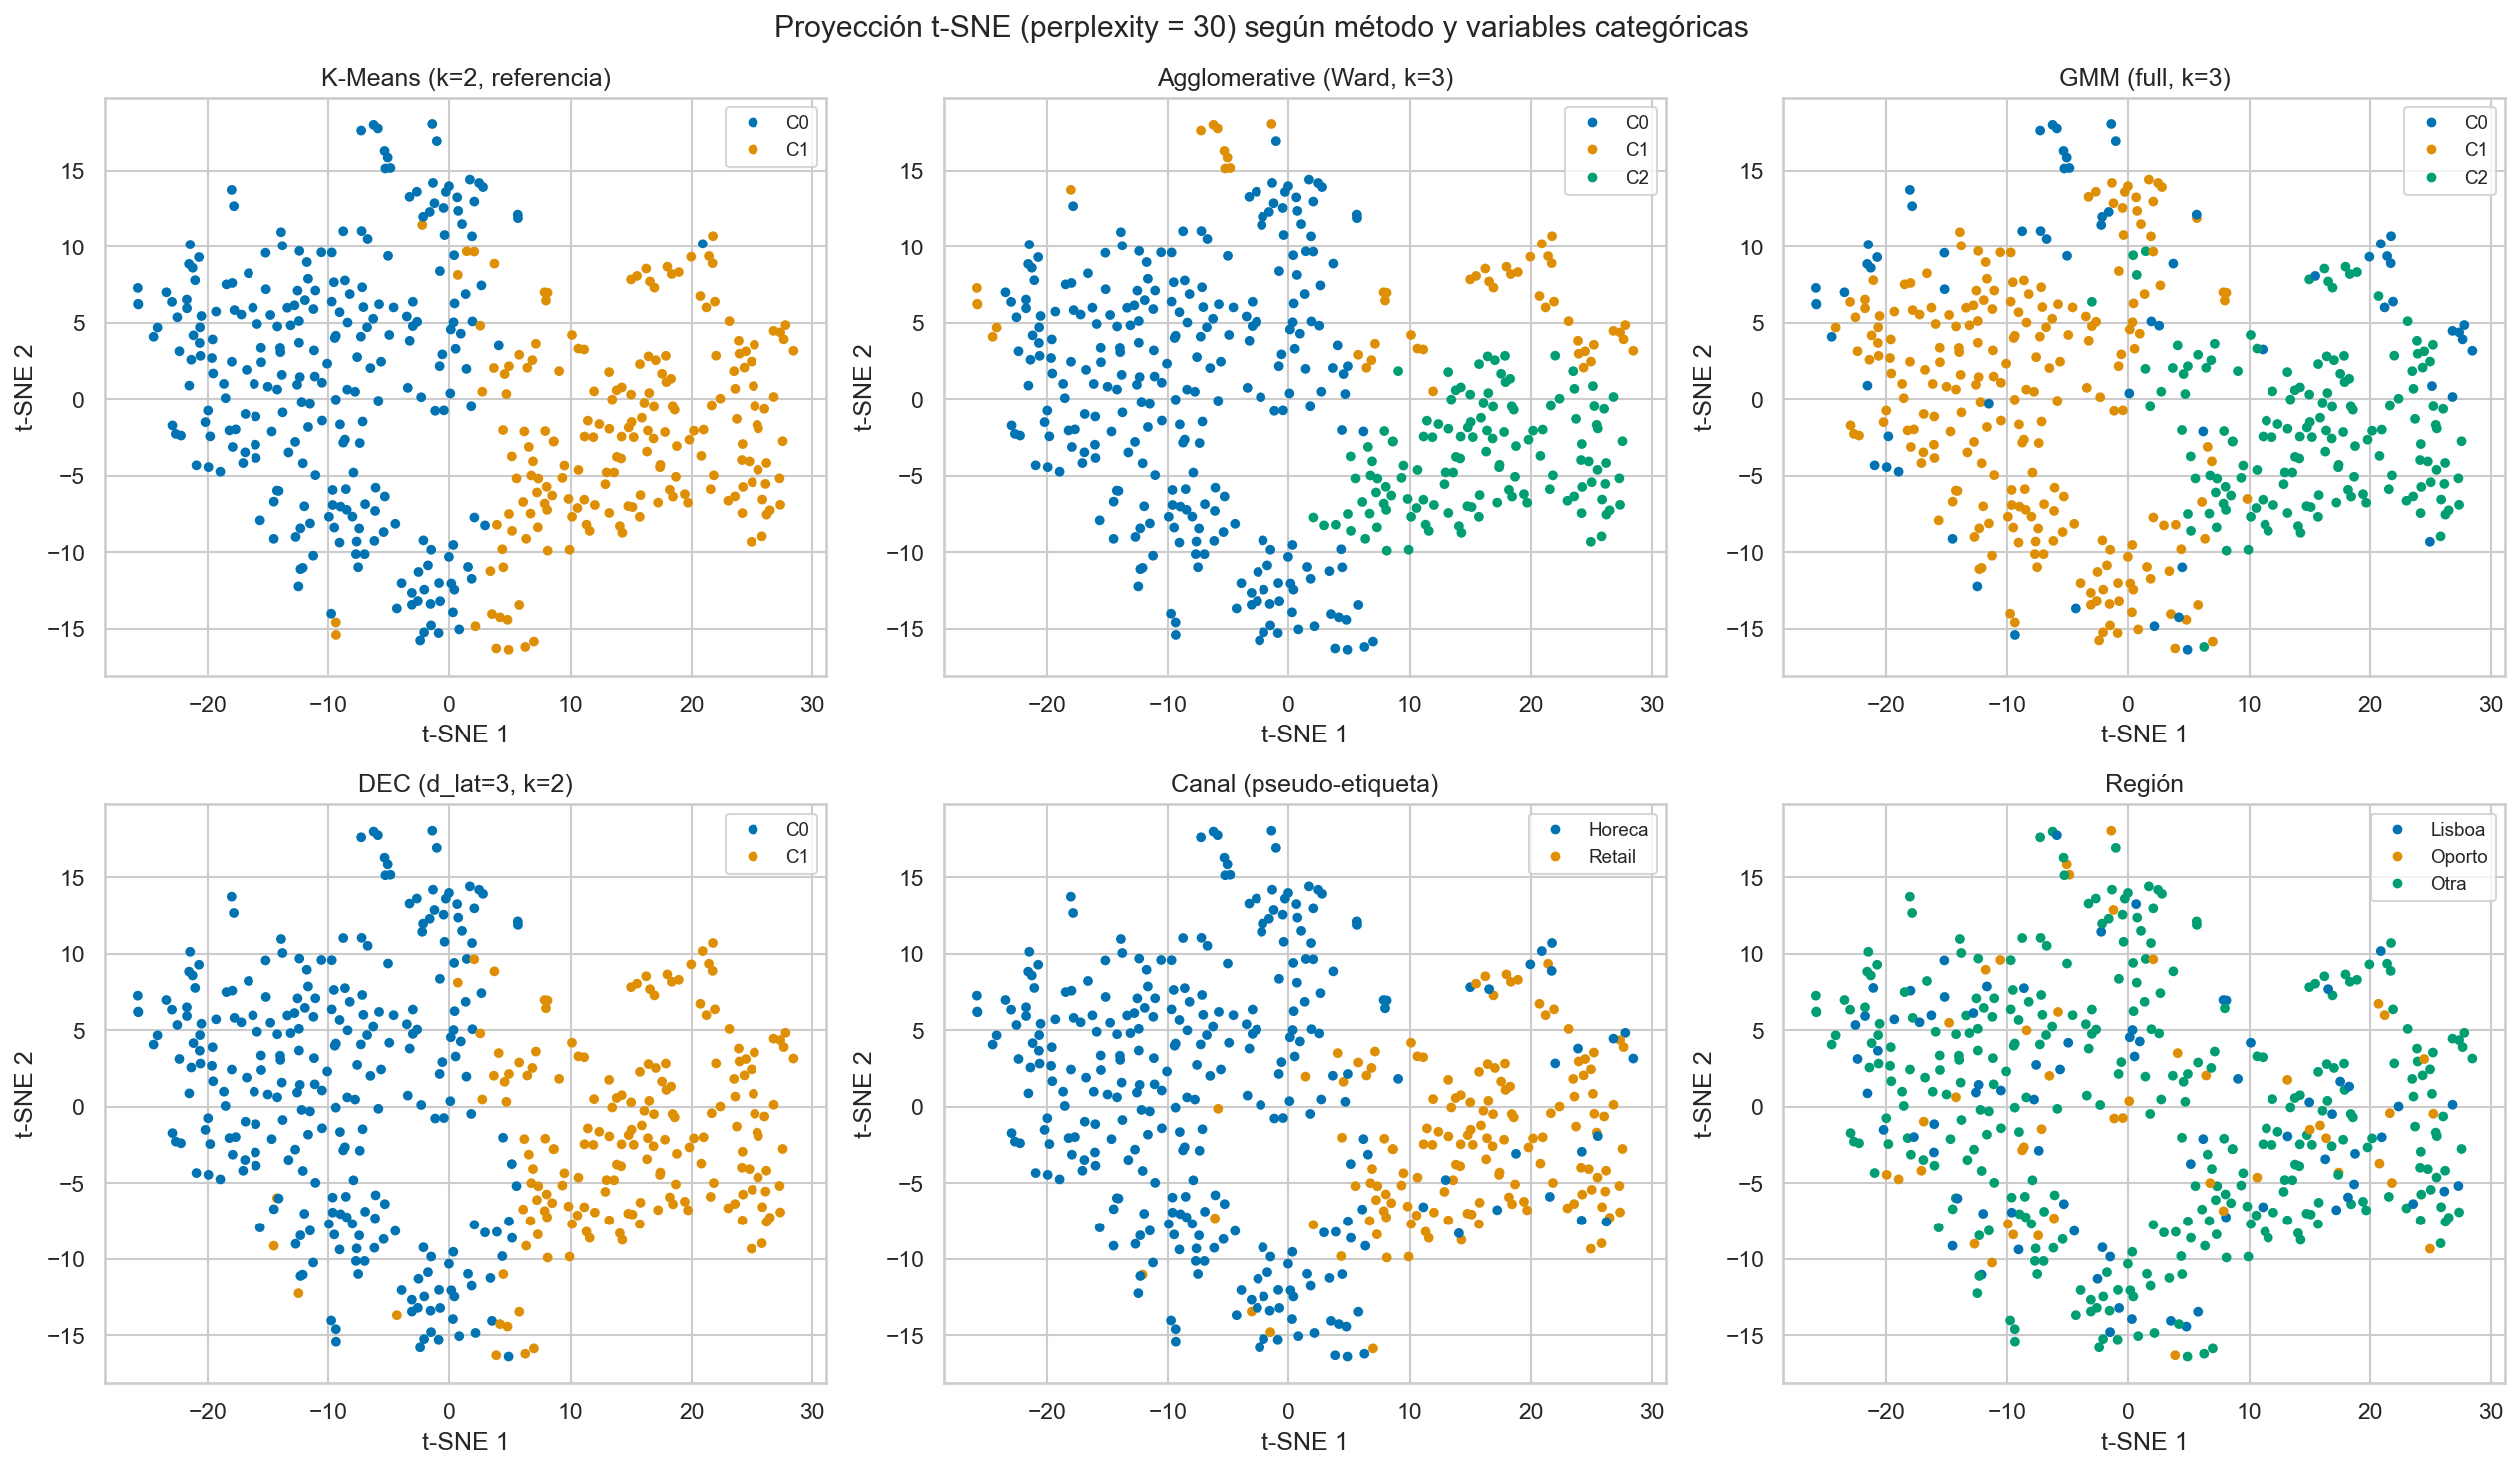
\includegraphics[width=0.94\textwidth,height=0.60\paperheight,keepaspectratio]{tsne_metodos.png}

  \vspace{0.1cm}
  \begin{columns}[T,onlytextwidth]
    \begin{column}{0.49\textwidth}
      {\footnotesize Dos regiones dominantes que coinciden con \highlight{Channel}, unidas por una zona de transici\'on sin frontera n\'itida: eso explica las \emph{silhouettes moderadas}.}
    \end{column}
    \begin{column}{0.49\textwidth}
      {\footnotesize El panel de \highlight{Region} no muestra patr\'on espacial: la estructura es \highlight{conductual, no geogr\'afica}. Los m\'etodos coinciden salvo el 3.\textsuperscript{er} grupo de Ward.}
    \end{column}
  \end{columns}
\end{frame}

% Guion: cerrar con decisiones de negocio, que es lo que queda en la memoria.
\begin{frame}{Insight de negocio: tres segmentos accionables}
  \begin{columns}[T,onlytextwidth]
    \begin{column}{0.57\textwidth}
      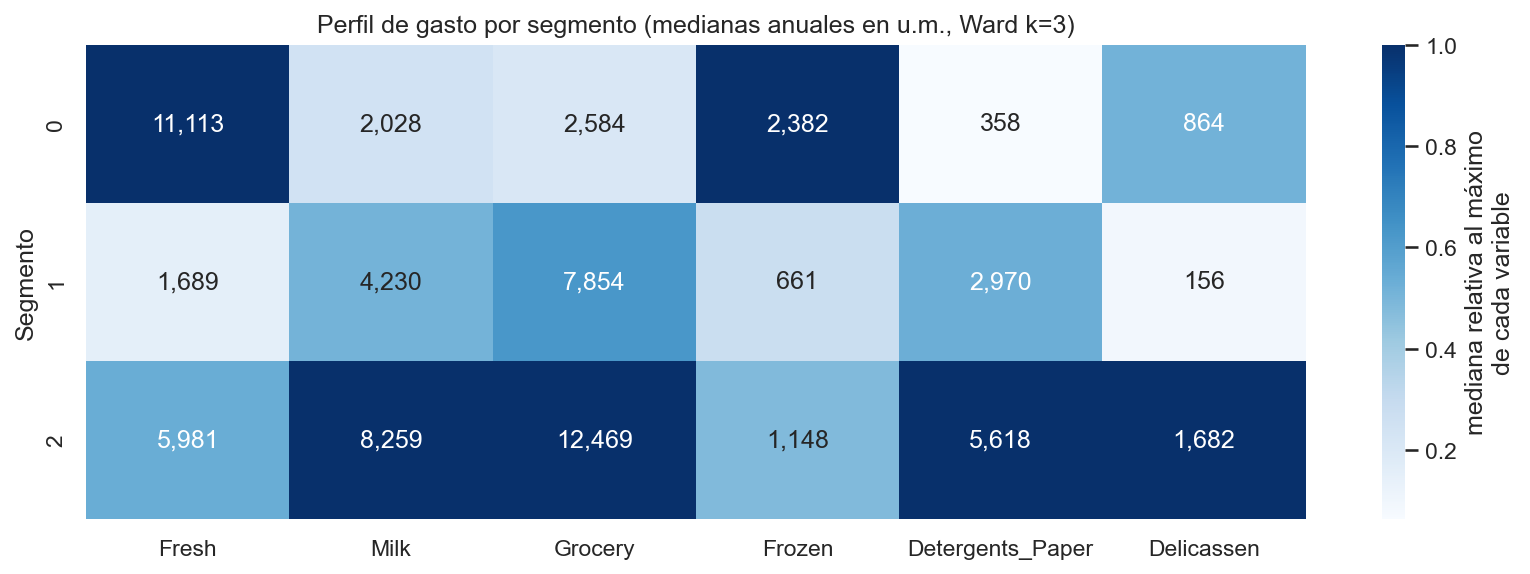
\includegraphics[width=\linewidth]{perfil_segmentos.png}
    \end{column}
    \begin{column}{0.40\textwidth}
      \begin{block}{Segmentos Ward k=3 \smallnote{(n=440)}}
        \begin{itemize}
          \item \textbf{0 - Frescos / Horeca} \smallnote{(262)}: prioridad en cadena de fr\'io y frecuencia de reparto.
          \item \textbf{1 - Reposici\'on bajo volumen / mixto} \smallnote{(53)}: candidato a desarrollo de cuenta y venta cruzada.
          \item \textbf{2 - Reposici\'on gran volumen / Retail} \smallnote{(125)}: foco en retenci\'on y condiciones comerciales.
        \end{itemize}
      \end{block}
    \end{column}
  \end{columns}

  \vspace{0.2cm}
  \centering
  \highlight{Conclusi\'on: el clustering transforma gasto hist\'orico en segmentos comerciales interpretables.}
\end{frame}

% Anexo: DEC en detalle; usar si preguntan por el metodo avanzado (deep clustering).
\begin{frame}{Anexo -- DEC: c\'omo funciona el deep clustering}
  \centering
  \resizebox{0.97\textwidth}{!}{%
  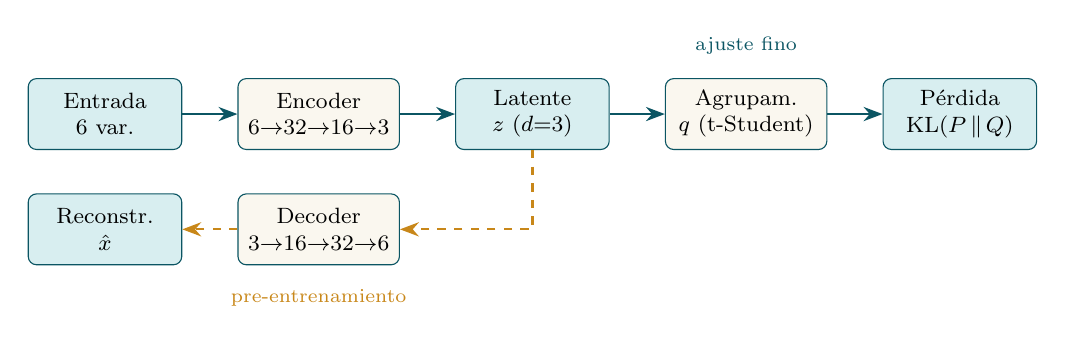
\begin{tikzpicture}[
    node distance=0.55cm and 0.7cm,
    box/.style={draw=DeepTeal, fill=SoftTeal, rounded corners=3pt, minimum width=1.95cm, minimum height=0.9cm, align=center, font=\footnotesize},
    ae/.style={draw=DeepTeal, fill=Paper, rounded corners=3pt, minimum width=2.05cm, minimum height=0.9cm, align=center, font=\footnotesize},
    arrow/.style={-{Stealth[length=2.4mm]}, thick, color=DeepTeal},
    darrow/.style={-{Stealth[length=2.4mm]}, thick, color=WarmAmber, dashed}
  ]
    \node[box] (x) {Entrada\\6 var.};
    \node[ae, right=of x] (enc) {Encoder\\$6{\to}32{\to}16{\to}3$};
    \node[box, right=of enc] (z) {Latente\\$z\ (d{=}3)$};
    \node[ae, right=of z] (clu) {Agrupam.\\$q$ (t-Student)};
    \node[box, right=of clu] (kl) {P\'erdida\\KL$(P\,\|\,Q)$};

    \draw[arrow] (x) -- (enc);
    \draw[arrow] (enc) -- (z);
    \draw[arrow] (z) -- (clu);
    \draw[arrow] (clu) -- (kl);

    \node[ae, below=of enc] (dec) {Decoder\\$3{\to}16{\to}32{\to}6$};
    \node[box, below=of x] (xhat) {Reconstr.\\$\hat{x}$};
    \draw[darrow] (z) |- (dec.east);
    \draw[darrow] (dec) -- (xhat);

    \node[font=\scriptsize, color=DeepTeal, above=0.18cm of clu] {ajuste fino};
    \node[font=\scriptsize, color=WarmAmber, below=0.18cm of dec] {pre-entrenamiento};
  \end{tikzpicture}%
  }

  \vspace{0.35cm}
  \begin{itemize}
    \footnotesize
    \item \highlight{Fase 1 (pre-entrenamiento):} el autoencoder comprime y reconstruye el gasto $\Rightarrow$ una representaci\'on latente $z$ que preserva la informaci\'on relevante.
    \item \highlight{Fase 2 (ajuste fino conjunto):} centroides inicializados con K-Means sobre $z$; se optimizan encoder y centroides minimizando $\mathrm{KL}(P\,\|\,Q)$ entre las asignaciones blandas $q$ y una distribuci\'on objetivo $P$ que las agudiza.
  \end{itemize}
  \smallnote{\textasciitilde2000 par\'ametros, full-batch y determinista; converge en segundos en CPU. Implementaci\'on en PyTorch siguiendo Xie et al. (2016).}
\end{frame}

% Anexo: respaldo tecnico para justificar la eleccion Ward k=3.
\begin{frame}{Anexo: dendrograma de Ward}
  \centering
  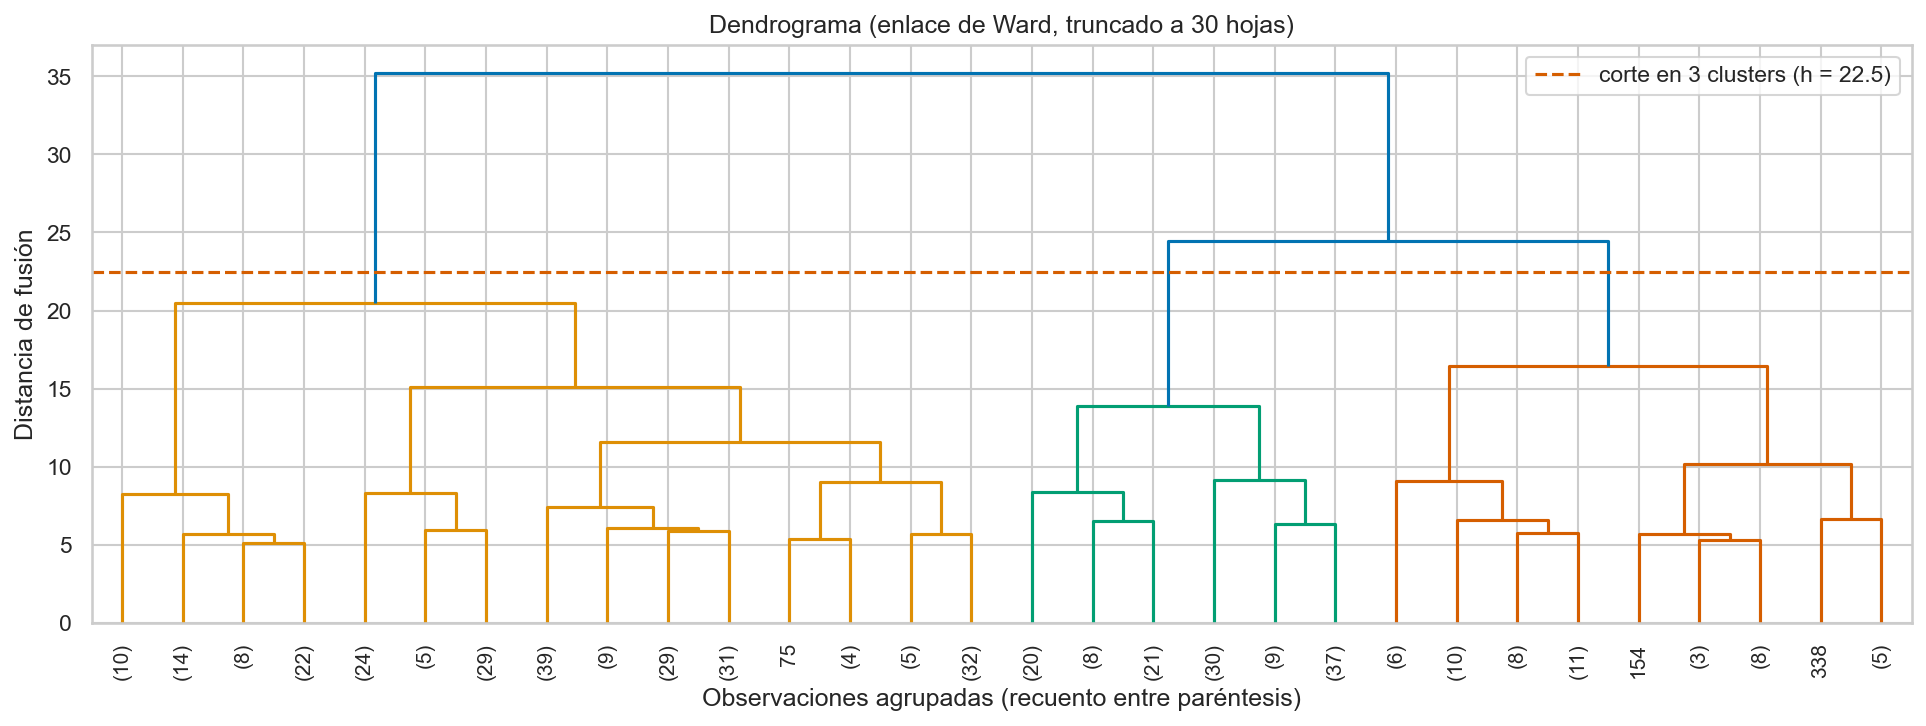
\includegraphics[width=0.98\textwidth,height=0.70\paperheight,keepaspectratio]{agglo_dendrograma.png}

  \vspace{0.12cm}
  \smallnote{Lectura: el corte marcado produce tres grupos, que luego se interpretan como segmentos comerciales accionables.}
\end{frame}

\end{document}
